\section{Wprowadzenie teoretyczne}

\subsection{Analiza wrażliwości}

Analiza wrażliwości jest kluczowym narzędziem w inżynierii konstrukcji, pozwalającym zrozumieć, jak zmiany parametrów wejściowych modelu wpływają na wynik analizowanego problemu.
W praktyce oznacza to, że można ocenić, które parametry - takie jak właściwości materiałowe, wymiary elementów czy obciążenia - mają największy wpływ na zachowanie się konstrukcji pod obciążeniem.
Dzięki temu jest możliwa zidentyfikacja potencjalnych słabości konstrukcji, zoptymalizować projekt pod kątem bezpieczeństwa i ekonomii, a także lepiej zarządzać ryzykiem związanym z niepewnościami w danych wejściowych.

Głównym celem analizy wrażliwości jest ilościowe określenie wpływu zmienności parametrów wejściowych na wybrane kryteria oceny konstrukcji, takie jak przemieszczenia, naprężenia czy ryzyko awarii.
W ten sposób, inżynierzy mogą podejmować świadome decyzje projektowe, uwzględniając nie tylko wartości nominalne parametrów, ale także ich potencjalne odchylenia.

Istnieje wiele metod stosowanych w analizie wrażliwości, różniących się podejściem i złożonością obliczeniową.
Do najpopularniejszych należą:

\begin{itemize}
    \item \textbf{Metoda różnic skończonych (Finite Difference Method)}: Polega na wprowadzeniu małych zmian w wartościach parametrów wejściowych i obserwacji, jak wpływają one na wynik. Jest to prosta metoda, ale może być czasochłonna przy dużej liczbie parametrów.
    \item \textbf{Metoda Monte Carlo}: Stosowana w analizach probabilistycznych, polega na losowym próbkowaniu wartości parametrów wejściowych i analizie wyników. Umożliwia ocenę rozkładu wyników oraz identyfikację najbardziej wpływowych parametrów.
    \item \textbf{Metoda współczynnika czułości (Sensitivity Coefficient Method)}: Oblicza względny wpływ zmiany parametru wejściowego na wynik. Jest to bardziej formalne podejście, które pozwala na dokładniejsze zrozumienie relacji pomiędzy parametrami a wynikami.
    \item \textbf{Metoda Sobola}: Zaawansowana technika, która rozkłada całkowitą wariancję wyników na poszczególne składowe, związane z różnymi parametrami wejściowymi. Pozwala to na ocenę zarówno efektów pojedynczych parametrów, jak i ich interakcji.
\end{itemize}

Analiza wrażliwości znajduje szerokie zastosowanie w inżynierii konstrukcji, szczególnie w kontekście:

\begin{itemize}
    \item Projektowania mostów i budynków pozwalając ocenić, jak zmienność właściwości materiałowych oraz różnorodność obciążeń wpływają na bezpieczeństwo i trwałość konstrukcji, co umożliwia podejmowanie świadomych decyzji projektowych.
    \item Analizy sejsmicznej, gdzie zrozumienie wrażliwości konstrukcji na parametry takie jak masa, sztywność, czy tłumienie jest kluczowe dla oceny ryzyka w przypadku trzęsienia ziemi.
    \item Optymalizacji projektów, umożliwiając identyfikację najbardziej krytycznych aspektów projektu, które mogą być zoptymalizowane w celu zwiększenia efektywności lub zmniejszenia kosztów.
\end{itemize}

\subsection{Losowość geometrii i właściwości materiałowych}

W inżynierii, nie da się uniknąć pewnych odchyłek od idealnych wartości, które są zakładane na etapie projektowania.
To właśnie ta nieprzewidywalność, która się nazywa losowością, może wynikać z wielu czynników.
Wahania w procesie produkcji mogą sprawić, że właściwości materiału, takie jak jego sprężystość czy wytrzymałość, będą się różnić w zależności od partii czy nawet drobnych zmian w procesie wytwarzania.

Do tego dochodzą zmiany w geometrii.
Nawet przy najlepszych intencjach, rzeczywiste wymiary elementów konstrukcyjnych mogą odbiegać od tych z projektu, choćby ze względu na tolerancje produkcyjne czy drobne błędy montażowe.
Nie należy też zapominać o warunkach, w jakich konstrukcja będzie pracować przez lata.
Czynniki zewnętrzne, takie jak korozja, zużycie czy zmiany temperatury, będą stopniowo wpływać na jej geometrię i właściwości materiału.

\subsubsection*{Losowość Geometrii}

Geometria konstrukcji jest szczególnie podatna na losowe odchylenia.
Tolerancje produkcyjne, błędy montażowe, a nawet długotrwała eksploatacja prowadząca do deformacji czy pęknięć - wszystko to sprawia, że rzeczywisty kształt konstrukcji może różnić się od tego, co założyliśmy na papierze.

Te, pozornie drobne, odchylenia mogą mieć znaczący wpływ na to, jak konstrukcja przenosi obciążenia.
Nierównomierny rozkład naprężeń, lokalne koncentracje naprężeń, a nawet utrata stabilności, szczególnie w przypadku smukłych elementów - to tylko niektóre z potencjalnych konsekwencji losowości geometrii.

\subsubsection*{Losowość właściwości materiałowych}

Podobnie jest z właściwościami materiałowymi.
Nawet jeśli na papierze materiał jest idealnie jednorodny, rzeczywistość może wyglądać inaczej.
Niejednorodność wynikająca z procesu produkcji, zmiany właściwości pod wpływem czynników środowiskowych, czy stopniowa degradacja materiału w czasie - wszystko to sprawia, że parametry takie jak moduł sprężystości, moment bezwładności czy wytrzymałość na rozciąganie mogą się różnić od wartości nominalnych.

\subsubsection*{Wpływ Losowości na analizę konstrukcji}

Pomijanie losowości w analizie konstrukcji stanowi istotne uproszczenie, które może prowadzić do niedoszacowania rzeczywistego ryzyka związanego z eksploatacją obiektu.
W praktyce, nieuniknione odchylenia od wartości nominalnych parametrów projektowych, wynikające zarówno z procesów produkcyjnych, jak i zmiennych warunków eksploatacyjnych, mogą znacząco wpłynąć na bezpieczeństwo i niezawodność konstrukcji.
Z tego względu, uwzględnienie losowości w procesie projektowania i analizy jest kluczowe dla zapewnienia odpowiedniego poziomu bezpieczeństwa.

Analiza probabilistyczna, która uwzględnia losowość parametrów, pozwala na ilościową ocenę ryzyka awarii lub przekroczenia stanów granicznych.
Dzięki temu możliwe jest projektowanie konstrukcji nie tylko spełniających wymagania wytrzymałościowe, ale przede wszystkim zapewniających odpowiedni poziom bezpieczeństwa, uwzględniający nieprzewidywalne czynniki.

Ponadto, uwzględnienie losowości może prowadzić do optymalizacji projektu pod kątem ekonomicznym i efektywnościowym.
Zamiast stosowania nadmiernych współczynników bezpieczeństwa, możliwe jest precyzyjne dostosowanie konstrukcji do rzeczywistych warunków eksploatacyjnych, co pozwala na oszczędność materiałów i zmniejszenie kosztów, przy jednoczesnym zachowaniu wymaganego poziomu bezpieczeństwa.

Analiza wrażliwości, będąca integralną częścią badania wpływu losowości, umożliwia identyfikację parametrów krytycznych, których zmienność ma największy wpływ na zachowanie konstrukcji.
Dzięki temu możliwe jest skoncentrowanie działań kontrolnych i zapobiegawczych na tych newralgicznych obszarach, minimalizując ryzyko i zapewniając długotrwałą i bezpieczną eksploatację obiektu.

\subsection{Metoda Monte Carlo}

Metoda Monte Carlo to niezwykle wszechstronne narzędzie numeryczne, pozwalające na badanie i rozwiązywanie problemów, w których niepewność i losowość odgrywają kluczową rolę.
W inżynierii, szczególnie w analizie wrażliwości konstrukcji, metoda Monte Carlo staje się niezastąpiona, umożliwiając ocenę wpływu zmienności różnych parametrów na zachowanie całej konstrukcji.

W skrócie, metoda Monte Carlo polega na wielokrotnym przeprowadzaniu symulacji, w których wartości parametrów wejściowych są losowane zgodnie z określonymi rozkładami prawdopodobieństwa\cite{montecarlo}.
Każda taka symulacja daje jeden wynik, a po zebraniu wielu takich wyników możliwe jest przeprowadzenie ich analizy statystycznej, co pozwala zrozumieć, jak różne czynniki wpływają na końcowy rezultat, na przykład na przemieszczenia czy naprężenia w konstrukcji.

Jak działa metoda Monte Carlo w analizie wrażliwości konstrukcji?
Proces ten można podzielić na kilka kluczowych etapów:

\begin{enumerate}
    \item \textbf{Identyfikacja parametrów losowych}: Na początku określane są parametry konstrukcji, które mogą podlegać losowości. Mogą to być właściwości materiału, takie jak moduł sprężystości, wymiary elementów konstrukcyjnych, a nawet wartości obciążeń zewnętrznych. Każdy z tych parametrów jest następnie opisywany za pomocą odpowiedniego rozkładu prawdopodobieństwa, który odzwierciedla jego zmienność.
    \item \textbf{Generowanie prób losowych}: Dla każdego zidentyfikowanego parametru generowane są losowe wartości zgodnie z jego rozkładem prawdopodobieństwa. Na przykład, jeśli moduł sprężystości materiału może się wahać w pewnym zakresie, to w każdej symulacji losowana jest jego wartość z tego zakresu.
    \item \textbf{Symulacja konstrukcji}: Mając zestaw losowo wygenerowanych parametrów, przeprowadzana jest symulacja zachowania konstrukcji pod obciążeniem. Można do tego wykorzystać na przykład metodę elementów skończonych (MES). Symulacja ta dostarcza informacji o tym, jak konstrukcja reaguje na zadane obciążenia, czyli jakie są przemieszczenia, naprężenia czy siły wewnętrzne w jej różnych elementach.
    \item \textbf{Powtórzenie symulacji}: Kroki 2 i 3 są powtarzane wielokrotnie, nawet tysiące czy miliony razy. Każde powtórzenie daje jeden wynik dla badanej wielkości, na przykład przemieszczenia w konkretnym punkcie konstrukcji.
    \item \textbf{Analiza statystyczna wyników}: Zebrane wyniki są następnie poddawane analizie statystycznej. Dzięki temu można uzyskać nie tylko pojedyncze wartości, ale cały rozkład prawdopodobieństwa dla badanej wielkości. Możliwe jest obliczenie wartości średniej, odchylenia standardowego, a nawet określenie prawdopodobieństwa, że wynik przekroczy pewien krytyczny poziom.
\end{enumerate}

\newpage
\subsubsection*{Zastosowanie metody Monte Carlo w analizie wrażliwości konstrukcji}
Metoda Monte Carlo jest szczególnie cenna w analizie wrażliwości konstrukcji, ponieważ umożliwia:

\begin{itemize}
    \item \textbf{Ocenę wpływu niepewności na wyniki}: Możliwa jest obserwacja, jak bardzo zmienność parametrów wpływa na zachowanie konstrukcji. Dzięki temu można określić, jakie są możliwe zakresy przemieszczeń czy naprężeń, a nie tylko ich wartości nominalne.
    \item \textbf{Identyfikację kluczowych parametrów}: Analiza wyników pozwala wskazać, które parametry mają największy wpływ na zmienność wyników. To pomaga skupić się na tych aspektach projektu, które są najbardziej krytyczne dla bezpieczeństwa i wydajności konstrukcji.
    \item \textbf{Zarządzanie ryzykiem}: Metoda Monte Carlo umożliwia przewidywanie i minimalizowanie ryzyka awarii konstrukcji. Jeśli wiadomo, które parametry są najbardziej niepewne, można odpowiednio dostosować projekt, zwiększając marginesy bezpieczeństwa lub wprowadzając dodatkowe środki kontroli.
\end{itemize}

\subsection{Rozkład normalny}

Rozkład normalny, znany również jako rozkład Gaussa, jest jednym z najważniejszych i najczęściej występujących rozkładów prawdopodobieństwa w statystyce i wielu dziedzinach nauki.
Jego charakterystyczny kształt dzwonu, symetryczny względem średniej, odzwierciedla tendencję wielu zjawisk naturalnych do skupiania się wokół wartości centralnej, przy jednoczesnym zmniejszaniu się prawdopodobieństwa wystąpienia wartości skrajnych.

W kontekście analizy wrażliwości konstrukcji, rozkład normalny znajduje szerokie zastosowanie do modelowania losowości parametrów, zarówno materiałowych, jak i geometrycznych.
Właściwości materiałów, takie jak moduł sprężystości czy wytrzymałość, a także wymiary elementów konstrukcyjnych, często wykazują naturalną zmienność wokół wartości średniej, którą można dobrze opisać właśnie rozkładem normalnym.

\begin{equation}
    f(x) = \frac{1}{\sigma \sqrt{2\pi}} e^{-\frac{(x - \mu)^2}{2\sigma^2}}\label{eq:gauss}
\end{equation}

\begin{figure}[H]
    \centering
    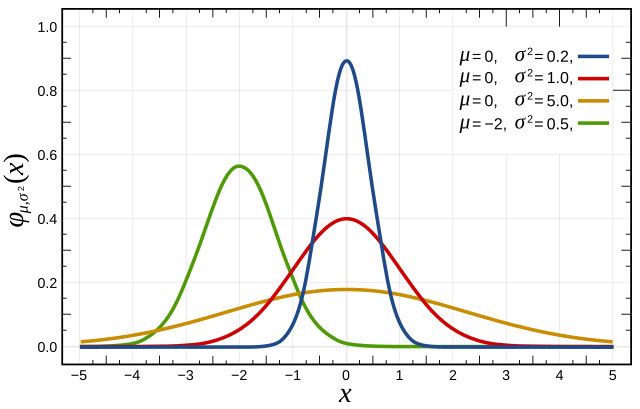
\includegraphics[scale=0.6]{images/Gauss}
    \caption{Rozkład Gaussa\cite{gauss}}
\end{figure}

Matematycznie, rozkład normalny jest opisany przez dwa parametry: średnią (\mu) oraz odchylenie standardowe (\sigma).
Średnia określa położenie środka rozkładu, a odchylenie standardowe określa jego szerokość, czyli jak bardzo wartości są rozproszone wokół średniej.
Im większe odchylenie standardowe, tym większa zmienność parametru\cite{gauss}.

Zastosowanie rozkładu normalnego w analizie wrażliwości konstrukcji przynosi szereg korzyści:

\begin{itemize}
    \item \textbf{Realistyczne modelowanie}: Pozwala na uwzględnienie naturalnej zmienności parametrów, co prowadzi do bardziej realistycznego odwzorowania rzeczywistych warunków.
    \item \textbf{Ilościowa ocena niepewności}: Dzięki znajomości średniej i odchylenia standardowego możliwe jest określenie prawdopodobieństwa wystąpienia różnych wartości parametru, co umożliwia ilościową ocenę niepewności.
    \item \textbf{Integracja z metodą Monte Carlo}: Rozkład normalny jest często wykorzystywany w metodzie Monte Carlo do generowania losowych wartości parametrów wejściowych, co umożliwia przeprowadzenie analizy probabilistycznej i ocenę wpływu zmienności parametrów na zachowanie konstrukcji.
\end{itemize}
W niniejszej pracy, rozkład normalny będzie stosowany do modelowania losowości wybranych parametrów materiałowych i geometrycznych konstrukcji prętowych.

\subsection{Metoda elementów skończonych MES}

Metoda elementów skończonych (MES) jest zaawansowaną techniką obliczeniową stosowaną do analizy i rozwiązywania problemów inżynierskich, w których wymagane jest zbadanie rozkładu naprężeń, przemieszczeń, temperatury czy innych parametrów fizycznych w konstrukcjach i materiałach.
MES polega na dyskretyzacji ciągłej przestrzeni, takiej jak belka, płyta czy bryła, na mniejsze, skończone elementy.
Każdy z tych elementów jest połączony z sąsiadującymi węzłami, które stanowią punkty, w których obliczane są wartości szukanych wielkości, takich jak przemieszczenia czy naprężenia\cite{trzylekcje}.

Podstawą działania metody elementów skończonych jest podział skomplikowanego problemu na wiele prostszych, łatwiejszych do rozwiązania części.
Cały obiekt inżynierski, na przykład most, jest dzielony na niewielkie, regularne elementy – trójkąty, czworokąty w przypadku problemów płaskich, lub czworościany i sześciany w przypadku problemów przestrzennych.
Każdy z tych elementów jest opisywany przez funkcje aproksymujące, które przybliżają rozkład szukanych wielkości na całym elemencie na podstawie wartości tych wielkości w węzłach elementu.

Kluczowym etapem w MES jest utworzenie macierzy sztywności, która reprezentuje zależności między obciążeniami działającymi na konstrukcję a przemieszczeniami w węzłach.
Macierz ta jest następnie używana do rozwiązania układu równań liniowych, który opisuje stan równowagi całej konstrukcji.
W zależności od liczby elementów oraz ich skomplikowania, układ równań może mieć bardzo dużą liczbę niewiadomych, co wymaga zastosowania odpowiednich algorytmów numerycznych oraz dużej mocy obliczeniowej.

\subsubsection{Równanie MES w statyce}

Równanie podstawowe w metodzie elementów skończonych (MES) w statyce, znane jako równanie równowagi, jest kluczowym narzędziem do analizy konstrukcji inżynierskich.
Jest to wyrażenie matematyczne, opisujące równowagę sił w konstrukcji, gdzie siły wewnętrzne (reprezentowane przez macierz sztywności i przemieszczenia) równoważą siły zewnętrzne.

\begin{equation}
\label{eq:mes}
    \bm{Kd} = \overline{\bm{r}}
\end{equation}
gdzie:

\begin{itemize}
    \item $\bm{K}$ - macierz sztywności globalnej konstrukcji
    \item $\bm{d}$ - wektor przemieszczeń węzłowych
    \item $\overline{\bm{r}}$ - wektor sił zewnętrznych działających na konstrukcję
\end{itemize}

Rozwiązanie tego równania pozwala na obliczenie przemieszczeń węzłowych, co z kolei umożliwia wyznaczenie naprężeń, odkształceń i innych, interesującyh projektanta, parametrów.

\subsubsection{Macierz sztywności}

Macierz sztywności reprezentuje relację między przemieszczeniami węzłowymi a siłami wewnętrznymi w konstrukcji.
Każdy element konstrukcji posiada swoją własną macierz sztywności elementu, która jest następnie składana w globalną macierz sztywności konstrukcji.

Macierz sztywności zależy od:

\begin{itemize}
    \item Właściwości materiałowych – Modułu Younga, współczynnika Poissona.
    \item Geometrii elementu – długości, przekroju poprzecznego.
    \item Typu elementu - belka, pręt, powłoka itp.
\end{itemize}

\subsubsection{Element belkowy}

Dla jednorodnej belki odkształcalnej w płaszczyźnie bez odkształceń osiowych posiadającej:

\begin{itemize}
    \item Cztery węzłowe stopnie swobody: poprzeczne przemieszczenie $w$ i obrót \theta na każdym końcu.
    \item Węzłowe siły $F_i$ i $F_j$ odpowiadają węzłowym przemieszczeniom $w_i$ i $w_j$.
    \item Węzłowe momenty $M_i$ i $M_j$ odpowiadają węzłowym obrotom $\theta_i$ i $\theta_j$.
\end{itemize}

W równaniu \ref{eq:mes}, gdzie K jest macierzą sztywności o wymiarach 4×4, a wektor węzłowych przemieszczeń elementu jest w postaci

\begin{equation}
\label{eq:ddsadadddd}
\macierz{d} =
    \begin{bmatrix}
        w_i & \theta_i & w_j & \theta_j
    \end{bmatrix}^T
\end{equation}

Wektor $\overline{\bm{r}}$ zawiera węzłowe siły i momenty przyłożone do elementu, tak aby utrzymać stan odkształcenia d.
Po rozpisaniu otrzymuje się

\begin{equation}
\label{eq:adadssadsssad}
\macierz{k} =
    \frac{EA}{L}
    \begin{bmatrix}
        k_{11} & k_{12} & k_{13} & k_{14} \\[1ex]
        k_{21} & k_{22} & k_{23} & k_{24} \\[1ex]
        k_{31} & k_{32} & k_{33} & k_{34} \\[1ex]
        k_{41} & k_{42} & k_{43} & k_{44} \\
    \end{bmatrix}
    \begin{bmatrix}
        w_i \\[1ex]
        \theta_i \\[1ex]
        w_j \\[1ex]
        \theta_j \\
    \end{bmatrix}
    =
    \begin{bmatrix}
        F_i \\[1ex]
        M_i \\[1ex]
        F_j \\[1ex]
        F_j \\
    \end{bmatrix}
\end{equation}

Aby wyrazić współczynniki sztywności w macierzy $\bm{k}$ w odniesieniu do geometrii elementu (moment bezwładności przekroju poprzecznego I, długość elementu L) oraz modułu sprężystości E, należy postępować w następujący sposób:

\begin{itemize}
    \item W celu wyznaczenia współczynników sztywności dla każdej kolumny macierzy $\bm{k}$, ustalamy odpowiednie stopnie swobody jako jednostkowe (równe 1), a pozostałe jako 0, po czym obliczamy siły ($F_i, F_j$) i momenty ($M_i, M_j$) niezbędne do uzyskania tego stanu deformacji.
    \item Pierwsza kolumna macierzy $\bm{k}$ jest wyznaczana przez aktywację tylko pierwszego stopnia swobody.
    \item Dla przypadku, gdy $w_i=1$ oraz $\theta_i=w_j=\theta_j=0$ z równania \ref{eq:ddsadadddd} otrzymuje się $k_{11}=F_i, k_{21}=M_i, k_{31}=F_j, k_{41}=M_j$.
\end{itemize}

Uznając belkę jako belkę wspornikową utwierdzoną z prawej strony i obciążoną z lewej strony i stosując równania teorii belek i statyki orzymuje się

\begin{equation}
\label{eq:asdadddddd1}
w=1 \quad \mathrm{węzeł} \quad i \quad  1=\frac{k_{11}L^3}{3EI}-\frac{k_{21}L^2}{2EI}
\end{equation}

\begin{equation}
\label{eq:asdadddddd2}
\theta=0 \quad \mathrm{węzeł} \quad i \quad  0=\frac{k_{11}L^2}{2EI}-\frac{k_{21}L}{EI}
\end{equation}

\begin{equation}
\label{eq:asdadddddd3}
\varSigma F=0 \qquad  0=k_{11}+k_{31}
\end{equation}


\begin{equation}
\label{eq:asdadddddd4}
\varSigma M=0  \qquad  0=k_{21}+k_{41}-k_{11}L
\end{equation}

Rozwiązanie tych równań wynosi:

\begin{equation}
\label{eq:asdaddasdaaaaadddd}
k_{11}=-k_{31}=\frac{12EI}{L^3} \quad i \quad k_{21}=k_{41}=\frac{6EI}{L^2}
\end{equation}

\begin{itemize}
    \item Współczynniki sztywności w kolumnach 2, 3 i 4 macierzy $\bm{k}$ wyznaczane poprzez podobny tok postępowania.
    \item Otrzymana macierz sztywności jest dokładna (nie przybliżona) pod warunkiem, że
pomija się poprzeczną deformacje na ścinanie, a przemieszczenia są małe.
    \item Po zdefiniowaniu macierzy sztywności względem parametrów E, I i L można rozwiązać problemy płaskich belek.
    \item Tworzenie modelu elementów skończonych wymaga przekształcenia obciążenia
rozłożonego w wektor obciążeń skupionych.
    \item Ponadto można połączyć macierze sztywności $\bm{k}$ dla pręta i dla belki, tak aby powstała
macierz sztywności o wymiarach 6×6, dla elementu ramowego, który posiada dwa
przemieszczenia translacyjne i jeden obrót na każdym końcu. Takie elementy mogą
być wykorzystywane do analizy ram płaskich.
\end{itemize}

Zakłąda się prosty elemenet belkowy o czterech stopniach swobody i że obrót \theta  jest mały, tak że
$\theta\approx dw/dx$.
Cztery stopnie swobody określają sześcienne pole przemieszczeń poprzecznych

\begin{equation}
\label{eq:ddaaaasadadddd}
\macierz{w} =
    N\begin{bmatrix}
        w_1 & \theta_1 & w_2 & \theta_2
    \end{bmatrix}^T
\end{equation}
Pole krzywizn dane jest wzorem $w_{xx}=Bd$, gdzie:

\begin{equation}
\label{eq:ddaaaasadad}
\macierz{B} =
    \frac{d^2}{dx^2}N=
    \begin{bmatrix}
        -\frac{6}{L^2}+\frac{12x}{L^3} & -\frac{-4}{L}+\frac{6x}{L^2} & \frac{6}{L^2}-\frac{12x}{L^3} & -\frac{-2}{L}+\frac{6x}{L^2}
    \end{bmatrix}
\end{equation}
Dla stałej sztywności giętnej EI, macierz sztywności elementu podana wzorem  ma następującą postać:

\begin{equation}
\label{eq:ddaaaasadadz}
\macierz{k} =
    \int^L_0 B^T EIBdx=
    \frac{EI}{L^2}
    \begin{bmatrix}
        12 & 6L & -12 & 6l \\[1ex]
        6L & 4L^2 & -6L & 2L^2 \\[1ex]
        -12 & -6L & 12 & -6l \\[1ex]
        6L & 2L^2 & -6L & 4L^2 \\
    \end{bmatrix}
\end{equation}

\subsubsection{Element ramowy}

Płaski element ramowy może odkształcić się osiowo (ściskanie lub rozciąganie) i poprzecznie (zginanie).
Tym samym, aby otrzymać charakterystyczne wektory i macierze płaskiego elementu ramowego możemy połączyć (wykonać superpozycję) elementu prętowego i belkowego.
Wówczas wektor węzłowych stopni swobody jest w postaci

\begin{equation}
\label{eq:ddddd}
\macierz{d} =
    \begin{bmatrix}
        u_1 & w_1 & \theta_1 & u_2 & w_2 & \theta_2
    \end{bmatrix}^T
\end{equation}

Jeśli element jest jednorodny i leży wzdłuż osi x, wówczas jego macierz sztywności ma postać

\begin{equation}
\label{eq:adadssssad}
\macierz{k} =
    \frac{EA}{L}
    \begin{bmatrix}
        1 & 0 & 0 & -1 & 0 & 0 \\[1ex]
        0 & 0 & 0 & 0 & 0 & 0 \\[1ex]
        0 & 0 & 0 & 0 & 0 & 0 \\[1ex]
        -1 & 0 & 0 & 1 & 0 & 0 \\[1ex]
        0 & 0 & 0 & 0 & 0 & 0 \\[1ex]
        0 & 0 & 0 & 0 & 0 & 0
    \end{bmatrix}
    +\frac{EI}{L^3}
    \begin{bmatrix}
        0 & 0 & 0 & 0 & 0 & 0 \\[1ex]
        0 & 12 & 6L & 0 & -12 & 6L \\[1ex]
        0 & 6L & 4L^2 & 0 & -6L & 2L^2 \\[1ex]
        0 & 0 & 0 & 0 & 0 & 0 \\[1ex]
        0 & -12 & -6L & 0 & 12 & -6L \\[1ex]
        0 & 6L & 2L^2 & 0 & -6L & 4L^2 \\
    \end{bmatrix}
\end{equation}

Ostatecznie macierz sztywności elementu ramowego według teorii Bernoulli-Eulera ma postać
\begin{equation}
\label{eq:adadad}
\macierz{k} =
    \begin{bmatrix}
        \frac{EA}{L} & 0 & 0 & -\frac{EA}{L} & 0 & 0 \\[1ex]
        0 & \frac{12EI}{L^3} & \frac{6EI}{L^2} & 0 & -\frac{12EI}{L^3} & \frac{6EI}{L^2} \\[1ex]
        0 & \frac{6EI}{L^2} & \frac{4EI}{L} & 0 & -\frac{6EI}{L^2} & \frac{2EI}{L} \\[1ex]
        -\frac{EA}{L} & 0 & 0 & \frac{EA}{L} & 0 & 0 \\[1ex]
        0 & -\frac{12EI}{L^3} & -\frac{6EI}{L^2} & 0 & \frac{12EI}{L^3} & -\frac{6EI}{L^{2}} \\[1ex]
        0 & \frac{6EI}{L^2} & \frac{2EI}{L} & 0 & -\frac{6EI}{L^2} & \frac{4EI}{L}
    \end{bmatrix}
\end{equation}

\subsection{Narzędzia programistyczne}
\subsubsection{Python}

Python, jako wszechstronny język programowania o otwartym kodzie źródłowym, cieszy się uznaniem w wielu dziedzinach\cite{python}.
Jego prosta i czytelna składnia, bogata biblioteka standardowa oraz dostępność licznych bibliotek zewnętrznych czynią go idealnym narzędziem do implementacji algorytmów analizy wrażliwości, przetwarzania danych oraz wizualizacji wyników.
W niniejszej pracy, Python został wykorzystany do automatyzacji procesu analizy, generowania modeli konstrukcji, przeprowadzania symulacji oraz przetwarzania i prezentacji wyników.

\subsubsection{OpenSees}

OpenSees (Open System for Earthquake Engineering Simulation) to zaawansowana platforma programistyczna o otwartym kodzie źródłowym, dedykowana symulacji zachowania konstrukcji pod wpływem obciążeń dynamicznych, w tym sejsmicznych\cite{opensees}.
Szeroki zakres dostępnych elementów skończonych, modeli materiałowych oraz algorytmów rozwiązywania sprawia, że OpenSees stanowi doskonałe narzędzie do analizy wrażliwości konstrukcji pr.
Integracja OpenSees z Pythonem umożliwiła płynną automatyzację procesu analizy, pozwalając na efektywne przeprowadzanie złożonych symulacji oraz dogłębną analizę wyników.